\chapter{Auswertung und Ergebnisse}
\label{chap.results}
\red[TODO:\\
PGFPlots einfügen\\
Daten aufbereiten\\
Ergebnisse vergleichen/auswerten\\
]

Um die Funktionalität des \kps{s} bewerten und verschiedene Anwendungsfälle vergleichen zu können wird eine experimentelle Evaluation durchgeführt. Diese soll besonders dazu dienen Fehlereinflüsse der einzelnen Schritte zwischen der Lokalisation des Systems und der Darstellung der visuelle Zusatzinformationen zu quantifizieren. Zunächst erfolgt eine Betrachtung der Lokalisationsgenauigkeit. Dazu wird die globale Lokalisation auf Basis der zwei in \kapitel{chap.globloc} beschriebenen Modelle durchgeführt. Anschließend erfolgt die Bestimmung der Fehlereinflüsse der visuellen Odometrie und der inertialen Messeinheit auf die lokale Positionsbestimmung. Abschließend wird eine gesonderte Betrachtung der Transformation zwischen Kamera und Projektor durchgeführt.\\
Als Bewertungsreferenz (Ground Truth) der Lokalisation werden die in \abb{fig.armarker} gezeigten Markerfelder verwendet.

\begin{figure}[!ht]
	\begin{center}
		
\includegraphics[scale=1.0]{spacer}
		\caption{AR Markerfelder}
		\label{fig.armarker}
	\end{center}
	%\vspace*{-8mm}
\end{figure}

Durch Erfassung in Kamerabildern können Orientierung und Ursprung der Felder bestimmt werden \red[näher erläuteren?]. Je Feld werden vier Marker aufgebracht um die Robustheit der Detektion zu erhöhen. Die jeweilige Positionierung der Felder ist abhängig von der jewiligen Untersuchung und wird innerhalb der folgenden Abschnitte detaillierter beschrieben. 

\section{Globale Lokalisation}
Die globale Lokalisation bildet die Basis der Positionsbestimmung. Dabei ist besonders eine approximative Bestimmung der Systempose von Bedeutung. Die Bestimmung einer möglichst exakten Annäherung der Pose ist zwar prinzipiell ebenso Ziel der globalen Lokalisation, kann jedoch bei korrekter initialer Approximation auch durch anschließende Optimierungsschritte erreicht werden. Im Falle einer fehlerhaften initialen Lokalisation kann trotz einer lokalen Optimierung nicht von einer Verringerung der Abweichung zur wahren Pose ausgegangen werden. Als zusätzliches Bewertungskriterium der globale Lokalisation wird deshalb im Folgenden neben der Abweichung zur realen Pose auch die Erfolgswahrscheinlichkeit der Approximation erfasst.\\

Um die wahre Pose des \kps{s} zu bestimmen wird das Markerfeld innerhalb der realen Umgebung auf einer glatten Fläche befestigt. Der Abgleich zwischen der daraus bestimmten Pose und der durch die Lokalisation ermittelten Pose ist dabei nur möglich, wenn die Pose des Markerfeldes auch in der Modellumgebung bekannt ist. Dies kann entweder durch Anbringung der Markerfelder vor der Kartierung oder durch Definition der Markerpose anhand eindeutiger Landmarken der Umgebung erreicht werden.\\

Die Bestimmung der Referenzpose kann nun durch Erfassung des Markerfeldes mit der Kamera des Systems erfolgen. Dazu wird das \kps{} in einer Pose fixiert und die Transformation zwischen dem Markerfeld und dem \kps{} bestimmt. Durch die vorhandene Verknüpfung zwischen der realen und der Modellumgebung ist die Transformation zwischen den Koordinatensystemen der Karte und des Markerfeldes beschrieben\red[ Bild?]. Es lässt sich somit die Transformation zwischen \kps{} und Karte bestimmen:

\begin{equation}
\tmat{M}{K} = \tmat{M}{AR}\tmat{AR}{K}
\end{equation}

Auch die globale Lokalisation wird durchgeführt während sich das \kps{} in der fixierten Pose befindet. Die so ermittelte Pose kann nun mit der Referenzposition verglichen werden. Im folgenden werden die Ergebnisse in Abhängigkeit des verwendeten Modells beschrieben. Die Fehlerwerte wurden dabei für alle Untersuchungen als Quadratischer Mittelwert über die Messungen bestimmt:

\begin{equation}
QMW = \sqrt{\frac{1}{n}\sum_{i=1}^nr_i^2}
\end{equation}

Aufgrund der Programmstruktur ist die Vorgabe eines Bereiches zur Verteilung der Partikel bezüglich der \red[z-Koordinate] der Karte erforderlich. Da das handgeführte \kps{} zu Beginn der Anwendung leicht in einer definierten Höhe bewegt werden kann, wurde dieser Grenzbereich mit einer Toleranz von $\pm$ \SI{0,1}{\meter} zur tatsächlichen Pose definiert.\\
\red[\abb{fig.error_glob_trans} zeigt den Vergleich der durch die beiden Modelle erzielten Fehlerwerte.\\]

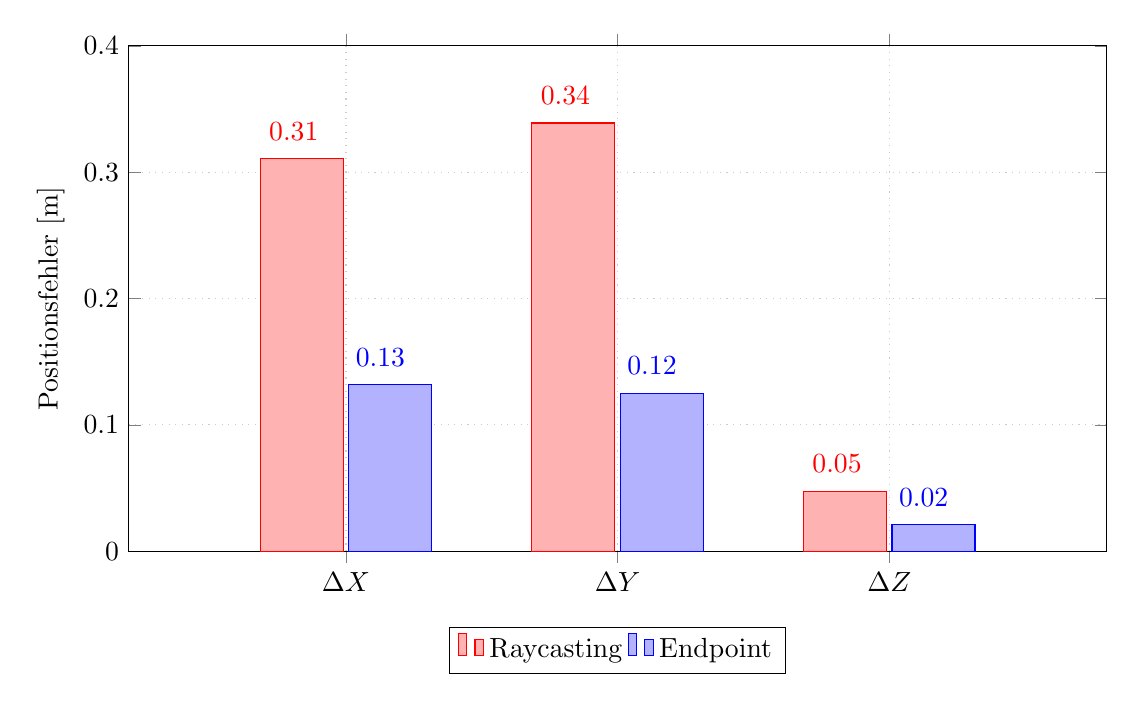
\begin{tikzpicture}
\begin{axis}[
	ybar,
	ymax=0.4,
	ymin=0,
	bar width=30pt,
	enlarge x limits=0.4,
	legend style={at={(0.5,-0.15)},
	anchor=north,legend columns=-1},
	ylabel={Positionsfehler \lbrack m\rbrack},
%	symbolic x coords={\Delta,y,z},
	xticklabels={$\Delta X$, $\Delta Y$, $\Delta Z$},
	xtick=data,
	every node near coord/.style={/pgf/number format/fixed, anchor=west},
	nodes near coords,
	nodes near coords align={vertical},
	width=14cm,
	height=8cm,
	grid=major,
    	grid style={dotted,lightgray!80!white},
    	scaled y ticks = false,
]
\addplot[
	every node near coord/.append style={xshift=-1.1cm},
	nodes near coords=\raisebox{0.7cm}{\pgfmathprintnumber\pgfplotspointmeta},
	color=red,
	fill=red!30!white
] coordinates {(-1,0.3105647208) (0,0.3388888731) (1,0.0473358078)};
\addplot[
	every node near coord/.append style={xshift=0.0cm},
	nodes near coords=\raisebox{0.7cm}{\pgfmathprintnumber\pgfplotspointmeta},
	color=blue,
	fill=blue!30!white
] coordinates {(-1,0.1315834135) (0,0.1248760865) (1,0.0209899568)};
\legend{Raycasting,Endpoint}
\end{axis}
\label{fig.error_glob_trans}
\end{tikzpicture}

\red[Winkelfehler Vergleich:\\]

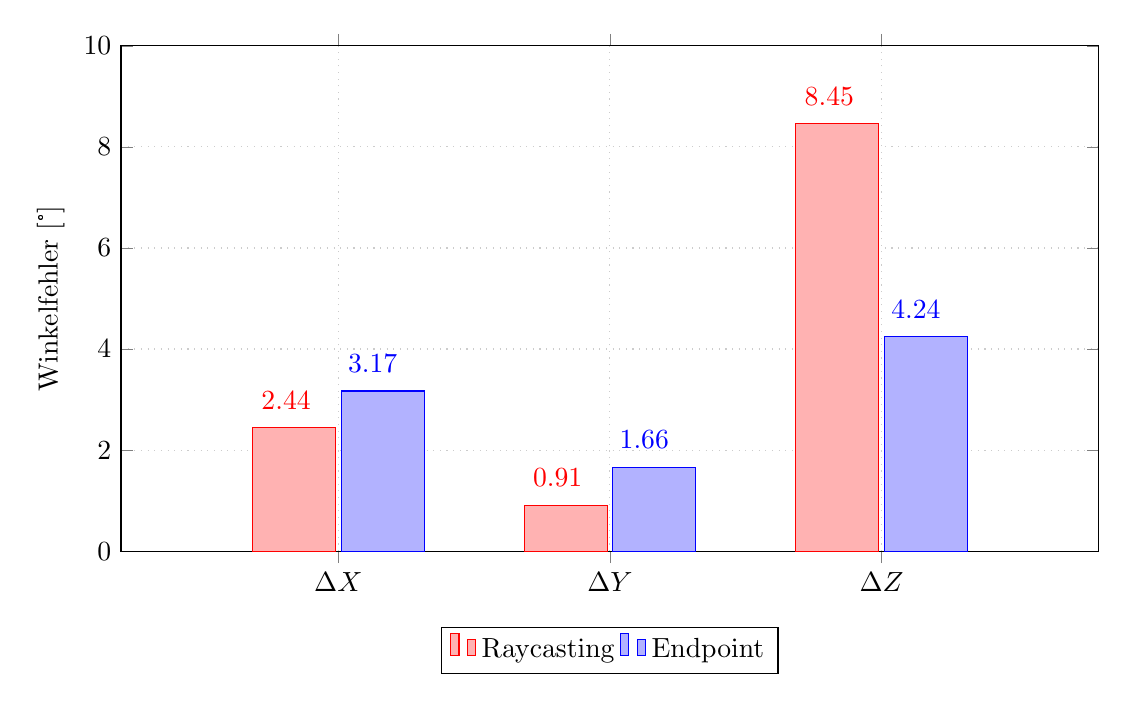
\begin{tikzpicture}
\begin{axis}[
	ybar,
	ymax=10,
	ymin=0,
	bar width=30pt,
%	enlarge y limits={0.4,upper},
	enlarge x limits=0.4,
	legend style={at={(0.5,-0.15)},
	anchor=north,legend columns=-1},
	ylabel={Winkelfehler \lbrack °\rbrack},
%	symbolic x coords={\Delta,y,z},
	xticklabels={$\Delta X$, $\Delta Y$, $\Delta Z$},
	xtick=data,
	every node near coord/.style={/pgf/number format/fixed, anchor=west},
	nodes near coords,
	nodes near coords align={vertical},
	width=14cm,
	height=8cm,
	grid=major,
    	grid style={dotted,lightgray!80!white},
    	scaled y ticks = false,
]
\addplot[
	every node near coord/.append style={xshift=-1.1cm},
	nodes near coords=\raisebox{0.7cm}{\pgfmathprintnumber\pgfplotspointmeta},
	color=red,
	fill=red!30!white
] coordinates {(-1,2.4445637073) (0,0.9069805767) (1,8.4545773848)};
\addplot[
	every node near coord/.append style={xshift=0.0cm},
	nodes near coords=\raisebox{0.7cm}{\pgfmathprintnumber\pgfplotspointmeta},
	color=blue,
	fill=blue!30!white
] coordinates {(-1,3.1694824628) (0,1.6633422885) (1,4.2398218425)};
\legend{Raycasting,Endpoint}
\end{axis}
\label{fig.error_glob_trans}
\end{tikzpicture}

Um die erfolgreiche Approximation der Pose zu bewerten wird wie in \abb{fig.loclimits} dargestellt ein Grenzraum um die wahre Position definiert. Darüber hinaus werden ebenfalls Grenzbereiche für die maximal zulässigen Winkelfehler festgelegt. Die zugehörigen Werte sind in \tab{thresh_glob} aufgeführt.\\

\begin{figure}[!ht]
	\begin{center}
		
\includegraphics[scale=1.0]{spacer}
		\caption{Grenzbereich der Lokalisation}
		\label{fig.loclimits}
	\end{center}
	%\vspace*{-8mm}
\end{figure}

\begin{table}[ht]
	\centering
	\caption{Grenzwerte zur Bestimmung der erfolgreichen Approximation}\label{tab.TechSpecYouBotBase}
	\vspace*{-3mm}
	\begin{tabular}[ht]{|l|r|}\hline
		\rowcolor{Snow2}
		Dimension		& Grenzwert 					\\ \hline
		X				& \SI{1}{\milli\meter}		\\ \hline		
		Y				& \SI{1}{\milli\meter}		\\ \hline
		Z				& \SI{1}{\milli\meter}		\\ \hline
		Yaw				& \SI{1}{\milli\meter}		\\ \hline
		Pitch			& \SI{1}{\milli\meter}		\\ \hline
		Roll 			& \SI{1}{\milli\meter}		\\ \hline		
		\hline
	\end{tabular} 
	\vspace*{-3mm}
\end{table}

\red[Quadratischer Mittelwert QMW statt Root Mean Square RMS überall aktualisieren]

\subsection{Raycasting-Modell}

\subsection{Endpoint-Modell}

\red[Relokalisation bei globaler Lokalisation beschreiben]

\section{Lokale Lokalisation}%Tracking/Kontinuierliche Lokalisation}
Die Genauigkeit der lokalen Lokalisations wird gesondert von der durch die globale Lokalisation bestimmten Pose betrachtet. Dazu wird ebenfalls das für die Untersuchung der globalen Lokalisation verwendete Markerfeld genutzt. Die wahre Pose des Systems kann so bestimmt und als Initialisierung der Lokalisation verwendet werden.\\
Die Bewertung der kontinuierlichen Lokalisation erfolgt gesondert für translatorische und rotatorische Bewegungen. Alle Messungen werden dabei separat durchgeführt um eine Beeinflussung der Bewegungen untereinander zu verhindern. Translatorisch werden dabei die Bewegung parallel (x-Achse der Kamera) und orthogonal (z-Achse der Kamera) zu einer Ebene betrachtet. Die parallele Bewegung wird dabei lediglich entlang einer Achse durchgeführt, da diese für beide Achsen parallel zur Ebene äquivalent ist und nur durch die Orientierung der Koordinatensysteme definiert wird. Ähnliches gilt für die Untersuchung der Lokalisationsgenauigkeit bei rotatorischen Bewegungen des Systems, da der Algorithmus der visuellen Odometrie nicht zwischen den Rotationsachsen der Kamera unterscheidet. Die Lokalisation während der Rotationsbewegungen wird zunächst allein auf Basis der visuellen Odometrie und anschließend allein auf Basis der inertialen Messeinheit durchgeführt. Abschließend erfolgt eine Bewertung der Lokalisation nach Fusion der beiden Sensorsysteme mittels des Erweiterten Kalman Filters.

\subsection{Translation X}

\subsection{Translation Z}

\subsection{Rotation Yaw}

\subsection{Rotation Pitch FOVIS}

\subsection{Rotation Roll FOVIS}

\subsection{Rotation Pitch IMU}

\subsection{Rotation Roll IMU}

\subsection{Rotation Pitch KALMAN}

\subsection{Rotation Roll KALMAN}

%Die globale Lokalisation wird anhand des Boards korrigiert um eine definierte Ausgangslage zu erhalten. Anschließend erfolgt eine Bewegung des Kamera-Projektor Systems entlang der verschiedenen Raumrichtungen und eine Rotation um die jeweiligen Winkel. Alle Messungen werden separat durchgeführt um eine Beeinflussung der Parameter untereinander zu verhindern. Die Bewegung erfolgt so, dass eine Rückkehr zur Ausgangslage stattfindet um eine Bestimmung der Positionsabweichung im Anschluss an die Bewegung durch erneute Detektion des Boards zu ermöglichen. Es ist darauf hinzuweisen, dass aufgrund der getrennten Betrachtung die Validierung zum einen für die visuelle Odometrie (x,y,z,yaw) und zum anderen für die Messdaten der IMU erfolgt (roll, pitch).

\section{Projektionsgenauigkeit}
Die Genauigkeit der Projektion virtueller Modelldaten wird unter Verwendung einer externen Kamera durchgeführt. Diese wird zunächst analog zum Vorgehen für die RGB-Kamera des Kinect Sensors kalibriert (siehe \kapitel{chap.calib}). Dadurch wird eine objektive Betrachtung der Projektionsgenauigkeit ermöglicht, da diese maßgeblich von der Kalibrierung des \kps{s} abhängt. Für die Untersuchung wird ein Markerfeld auf einer ebenen Unterlage fixiert und im Sichtfeld der RGB-Kamera des Kinect Sensors platziert. Durch die Erfassung des Markerfeldes und der daraus bestimmten Transformation kann die Position des \kps{s} relativ zum Markerfeld bestimmt werden.\red[ Markerfelder abbilden? Erstes Oben schon, zweites hier?]\\

Die bekannte Transformation zwischen Kamera- und Projektorkoordinaten ermöglicht nun die Zuordnung der detektierten 3D-Koordinaten des Markerfeldes zu den 2D-Koordinaten des Projektorbildes. Um die Projektionsgenauigkeit zu überprüfen wird nun mittels des Projektors ein weiteres Markerfeld projiziert, welches bezogen auf die Projektorkoordinaten deckungsgleich mit dem realen Markerfeld ist. \red[\abb{fig.arprojected}]\\

\begin{figure}[!ht]
	\begin{center}
		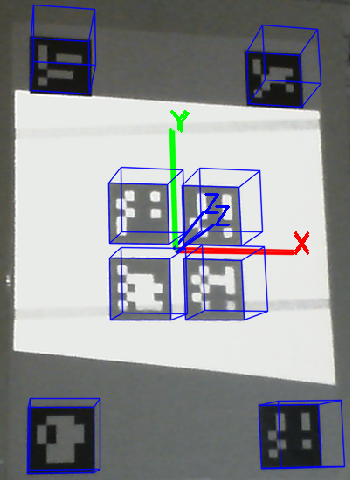
\includegraphics[scale=0.5]{board_eval_cropped}
		\caption{AR Marker real und projiziert}
		\label{fig.arprojected}
	\end{center}
	%\vspace*{-8mm}
\end{figure}

Die externe Kamera wird nun eingesetzt, um beide Markerfelder gleichzeitig zu erfassen und die Abweichungen zwischen den Feldern bezüglich Position und Orientierung zu bestimmen. Dabei werden die Positionierungen sowohl des \kps{s} als auch der externen Kamera während der Untersuchungen variiert. \red[Die Bestimmung der Fehlerwerte erfolgt erneut über Berechnung des QMW.\\
Die Ergebnisse der $n=6$ Messreihen sind in \tab{projection} zusammengefasst.]\\
Der Box-Whisker-Plot in \abb{fig.boxplot_proj} zeigt die Verteilung der translatorischen Fehlerwerte entlang der Raumachsen.\\

\begin{figure}
\begin{center}
\begin{tikzpicture}[trim axis left, trim axis right]
  \begin{axis}[
    	ytick={-30,-20,...,30},
    		minor y tick num=3,
    		ymax=35,
    		ymin=-35,
    		ylabel=Y-Achse \lbrack mm\rbrack,
    		xtick={1,...,3},
    		x tick label style={align=center},
    		xticklabels={$\Delta X$,$\Delta Y$,$\Delta Z$},
    		boxplot/draw direction=y,
    		width=14cm,
    		height=8cm,
    		grid=major,
    		grid style={dotted,lightgray!80!white},
    ]
    \addplot+[color=red,mark=x,
    		boxplot prepared={
      		lower whisker=-7.2937458753,
      		lower quartile=-2.2697057575,
      		median=-0.5078930408,
      		upper quartile=2.5787912309,
      		upper whisker=5.2836090326,
      		box extend=0.5,
    		},
    ] coordinates {};
    %table[row sep=\\,y index=0] {0.0\\}; %Ausreisser
    \addplot+[color=Green,mark=x,
    		boxplot prepared={
      		lower whisker=-5.6481547653,
      		lower quartile=0.8273310959,
      		median=2.7935747058,
      		upper quartile=6.1452584341,
      		upper whisker=6.959207356,
			box extend=0.5,
		},
    ] coordinates {};
    %table[row sep=\\,y index=0] {0.0\\}; %Ausreisser
    \addplot+[color=blue,mark=x,
    		boxplot prepared={
      		lower whisker=-30.851304531,
      		lower quartile=-12.757569552,
      		median=5.149245262,
      		upper quartile=11.0025405888,
      		upper whisker=22.670924664,
%      		lower whisker=-9.7615455743,
%      		lower quartile=-4.0365747411,
%      		median=1.6292533837,
%      		upper quartile=3.4812726082,
%      		upper whisker=7.173222257,
			box extend=0.5,
		},
    ] coordinates {};
    %table[row sep=\\,y index=0] {0.0\\}; %Ausreisser
  \end{axis}
\end{tikzpicture}
\caption{Box-Whisker-Plot}
\label{fig.boxplot_proj}
\end{center}
\vspace{-3mm}
\end{figure}

\red[Öffnungswinkel $\sim$ 30°, dadurch Faktor 16/9 für Fehlerwerte in z-Richtung. Sogar (16/9)² für Detektion+Projektion? Dann würden sich die Werte auf jeden Fall stark annähern]

\red[Nennen, dass Boxplot ganze Messreihe abbildet! Oder umwandeln zu 5/95 Perzentil?\\]

\begin{table}[ht]
	\centering
	\caption{Technische Daten der youBot Plattform}\label{tab.TechSpecYouBotBase}
	\vspace*{-3mm}
	\begin{tabular}[ht]{|l|c|r|}\hline
		\rowcolor{Snow2}
		Bezeichnung						& Formelzeichen	& \\ \hline
		Gesamtlänge 					&			& \SI{530}{\milli\meter}				\\ \hline
		Gesamtbreite 					&  		& \SI{350}{\milli\meter}				\\ \hline
		Höhe									&  		& \SI{106}{\milli\meter}				\\ \hline
		Radstand							& $l$	& \SI{470}{\milli\meter}				\\
		\hline
	\end{tabular} 
	\vspace*{-3mm}
\end{table}


%Überprüfung der Genauigkeit mit Hilfe externer Kamera. Externe Kamera wird kalibriert um objektive Betrachtung der Projektionsgenauigkeit zu ermöglichen. Kamera Projektor System ist bereits kalibriert. Verwendung von 2 QR Boards. Eins wird auf ebene Unterlage aufgeklebt, das andere wird vom Projektor projiziert. Zunächst wird das aufgeklebte Board durch die Kamera des Kamera Projektor Systems erkannt um daraus die Transformation zu berechnen, welche im Programm verwendet wird um die Projektorsicht zu erzeugen. Das projizierte Board wird anschließend mit der externen Kamera erfasst genauso wie das aufgeklebt. Es wird jeweils die Transformation zur Kamera berechnet um daraus die Differenz der beiden Boards bezüglich Position und Lage zu bestimmen.

\section{Benutzerinteraktion}

\begin{figure}[!ht]
\vspace{3mm}
\begin{center}
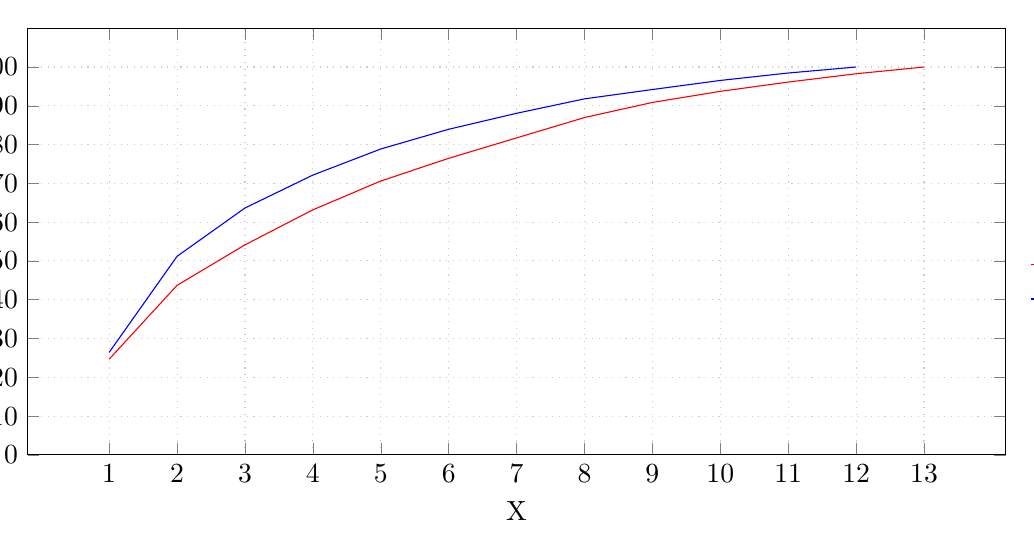
\begin{tikzpicture}[trim axis left, trim axis right]
	\begin{axis}[
		xlabel=X,
		ylabel=Y,
		xtick={1,...,13},
		ymin=0,
		ytick={0,10,...,100},
		legend style={
			at={(1,0.5)},
			xshift=0.2cm,
			anchor=north west,
			nodes=right,
			draw=none
		},
		grid=major,
   		grid style={dotted,lightgray!80!white},
		%axis lines=left
		width=14cm,
		height=7cm,
	]
	\addplot[color=red] coordinates{
		(1,24.6718)
		(2,43.7092)
		(3,54.14785132)
		(4,63.1821339)
		(5,70.60866985)
		(6,76.45681086)
		(7,81.7263871)
		(8,86.97406846)
		(9,90.86684525)
		(10,93.72329021)
		(11,96.11621437)
		(12,98.25885879)
		(13,100)		
	};
	\addplot[color=blue] coordinates{
		(1,26.42529337)
		(2,51.19458535)
		(3,63.64859236)
		(4,72.13773673)
		(5,78.8676646)
		(6,83.94694845)
		(7,88.06842906)
		(8,91.7882484)
		(9,94.19470806)
		(10,96.53607266)
		(11,98.45170481)
		(12,100)
		
	};
	\legend{Testa,Testb}
	\end{axis}
\end{tikzpicture}
\end{center}
\vspace{-3mm}
\caption{test1}
\label{fig.test1}
\vspace{3mm}
\end{figure}

\begin{figure}[ht]
\centering
\begin{tikzpicture}
\begin{axis}[
xlabel={Zeit},
ylabel={Position},
ymin=0,
ymax=6,
width=100mm,
height=80mm,
ytick={0,1,...,5},
legend style={at={(1,1)},	anchor=north east, xshift=-1mm,	yshift=-1mm}
]
\pgfplotstableread{plot/test.txt}\datatable
\addplot[color=red,mark=square*] table[x index=0,y index=1] from \datatable;
%\addplot[no markers] table[x index=0,y index=3] from \datatable;
%\addplot[no markers] table[y = Leistung] {plot/test.txt}  ;
\legend{test}
\end{axis}
\end{tikzpicture}
\caption{test2}
\label{fig.test2}
\end{figure}

\begin{figure}
\begin{center}
\begin{tikzpicture}[trim axis left, trim axis right]
  \begin{axis}[
    	ytick={0,0.1,...,1.1},
    		minor y tick num=5,
    		ymax=1.1,
    		ylabel=Y-Achse,
    		xtick={1,...,4},
    		x tick label style={align=center},
    		xticklabels={A, B},
    		boxplot/draw direction=y,
    		width=8cm,
    		height=8cm,
    		thick,
    ]
%    \addplot+[color=red,mark=x,
%    		boxplot prepared={
%      		lower whisker=,
%      		lower quartile=,
%      		median=,
%      		upper quartile=,
%      		upper whisker=
%    		},
%    ] %coordinates {};
%    table[row sep=\\,y index=0] {0.7054\\ 0.9773\\  0.9763\\ 0.9698\\ 0.7118\\ 0.6919\\ 0.9727\\ 0.7006\\ 0.974\\ 0.7077\\}; %Ausreisser
    \addplot+[color=Green,mark=x,
    		boxplot prepared={
      		median=0.3036,
      		upper quartile=0.34925,
      		lower quartile=0.2674,
      		upper whisker=0.5597,
      		lower whisker=0.18718
		},
    ] %coordinates {};
    table[row sep=\\,y index=0] {0.6045\\ 0.1818\\ 0.5826\\ 0.5688\\ 0.1814\\ 0.1825\\ 0.5750\\ 0.1783\\ 0.6312\\ 0.1793\\}; %Ausreisser
  \end{axis}
\end{tikzpicture}
\caption{Box-Whisker-Plot}
\label{fig.error_boxplot}
\end{center}
\vspace{-3mm}
\end{figure}